%Lab report on translation, scaling and shearing
\documentclass[12pt]{article}

\usepackage{amsmath}
\usepackage{graphicx}
\usepackage[a4paper]{geometry}

\geometry{
  textwidth=\dimexpr\paperwidth-29mm,
  textheight=\dimexpr\paperheight-32mm,
  noheadfoot,
  nomarginpar
}

\setlength{\topskip}{0mm}
\setlength{\parindent}{0mm}

\title{Translation, Scaling and Shearing}
\date{}
\author{}

\begin{document}
	\maketitle
	\vspace{-2cm}

	\section{Objective}
	To implement translation, scaling and shearing on given objects represented by their vertices.
	\section{Theory}
	\subsection{Translation}
	Translation is the process of moving an object from one position to another. The object is translated by adding the translation vector to the coordinates of each vertex of the object. The translation vector is given by
	\begin{equation*}
		\begin{bmatrix}
			t_x\\
			t_y
		\end{bmatrix}
	\end{equation*}
	\subsection{Scaling}
	Scaling is the process of changing the size of an object. The object is scaled by multiplying the coordinates of each vertex of the object by the scaling factor. The scaling factor is given by
	\begin{equation*}
		\begin{bmatrix}
			s_x\\
			s_y
		\end{bmatrix}
	\end{equation*}
	\subsection{Shearing}
	Shearing is the process of changing the shape of an object. The object is sheared by adding a multiple of one coordinate to the other coordinate of each vertex of the object. The shearing factor is given by
	\begin{equation*}
		\begin{bmatrix}
			sh_x\\
			sh_y
		\end{bmatrix}
	\end{equation*}

	\section{Algorithm}
	\subsection{Translation}
	\begin{enumerate}
		\item Read the coordinates of the object.
		\item Read the translation vector.
		\item Add the translation vector to the coordinates of each vertex of the object.
		\item Plot the translated object.
	\end{enumerate}
	\subsection{Scaling}
	\begin{enumerate}
		\item Read the coordinates of the object.
		\item Read the scaling factor.
		\item Multiply the coordinates of each vertex of the object by the scaling factor.
		\item Plot the scaled object.
	\end{enumerate}
	\subsection{Shearing}
	\begin{enumerate}
		\item Read the coordinates of the object.
		\item Read the shearing factor.
		\item Add a multiple of one coordinate to the other coordinate of each vertex of the object.
		\item Plot the sheared object.
	\end{enumerate}

	\section{Source Code}

\begin{verbatim}
#include <graphics.h>

// translate to the axes defined by the computer
void translateAxes(int *x, int *y)
{
    *x = (*x + WIDTH/2);
    *y = (- *y + HEIGHT/2);
}
void drawTriangle(int coordinates[3][2])
{
    int copy[3][2];
    for(unsigned i = 0; i<3; i++)
    {
        copy[i][0] = coordinates[i][0];
        copy[i][1] = coordinates[i][1];
    }
    for(unsigned i = 0; i<3; i++) 
        translateAxes(&copy[i][0], &copy[i][1]);
    // plot the translated points
    for(unsigned i = 0; i<3; i++) 
        line(copy[i][0], copy[i][1], copy[(i+1)%3][0], copy[(i+1)%3][1]);
}

void drawObject(unsigned num_points, int coordinates[][2])
{
    int copy[num_points][2];
    for(unsigned i = 0; i<num_points; i++)
    {
        copy[i][0] = coordinates[i][0];
        copy[i][1] = coordinates[i][1];
    }
    for(unsigned i = 0; i<num_points; i++)
        translateAxes(&copy[i][0], &copy[i][1]);
    // plot the translated points
    for(unsigned i = 0; i<num_points; i++)
       line(copy[i][0], copy[i][1], copy[(i+1)%num_points][0], copy[(i+1)%num_points][1]);
}

void scale(unsigned num_points, int coordinates[][2], float sx, float sy, int axis[2])
{
    for (unsigned i = 0; i < num_points; i++)
    {
        coordinates[i][0] = axis[0] + (coordinates[i][0] - axis[0]) * sx;
        coordinates[i][1] = axis[1] + (coordinates[i][1] - axis[1]) * sy;
    }
}

void shearX(unsigned num_points, int coordinates[][2], float shx, int ref)
{
    for (unsigned i = 0; i < num_points; i++)
    {
        coordinates[i][0] = coordinates[i][0] + (coordinates[i][1] - ref) * shx;
    }
}

void shearY(unsigned num_points, int coordinates[][2], float shy, int ref)
{
    for (unsigned i = 0; i < num_points; i++)
    {
        coordinates[i][1] = coordinates[i][1] + (coordinates[i][0] - ref) * shy;
    }
}

void translate(unsigned num_points, int coordinates[][2], int tx, int ty)
{
    for (unsigned i = 0; i < num_points; i++)
    {
        coordinates[i][0] += tx;
        coordinates[i][1] += ty;
    }
}

int main()
{   
    int gd = DETECT, gm;
    initgraph(&gd, &gm, "");
    setcolor(GREEN);
    
    // coordinates of a triangle in the first quadrant
    int triangle[3][2] = 
    {
        {-50, 0},
        {-100, -100},
        {-50, -100}
    };
    int axis[2] = {0, 0};

    // translation stuff
    cleardevice();
    outtextxy(WIDTH/2, 10, "Translation");
    drawTriangle(triangle);
    translate(3, triangle, 100, 0);
    drawTriangle(triangle);
    delay(2000);

    // scaling stuff
    cleardevice();
    outtextxy(WIDTH/2, 10, "Scaling");
    drawTriangle(triangle);
    scale(3, triangle, 0.6, 0.6, axis);
    drawTriangle(triangle);
    delay(2000);

    // shearing stuff
    cleardevice();
    outtextxy(WIDTH/2, 10, "Shearing");

    int square[][2] = 
    {
        {0, 0},
        {100, 0},
        {100, 50},
        {0, 50}
    };
    drawObject(4, square);
    delay(1000);

    shearX(4, square, 2, 0);
    drawObject(4, square);
    delay(1000);
    cleardevice();

    getch();
    closegraph();
    return 0;
}

\end{verbatim}

	\newpage
	\section{Output}

	\begin{figure}[!ht]
		\hspace*{-1cm}
		\centering
		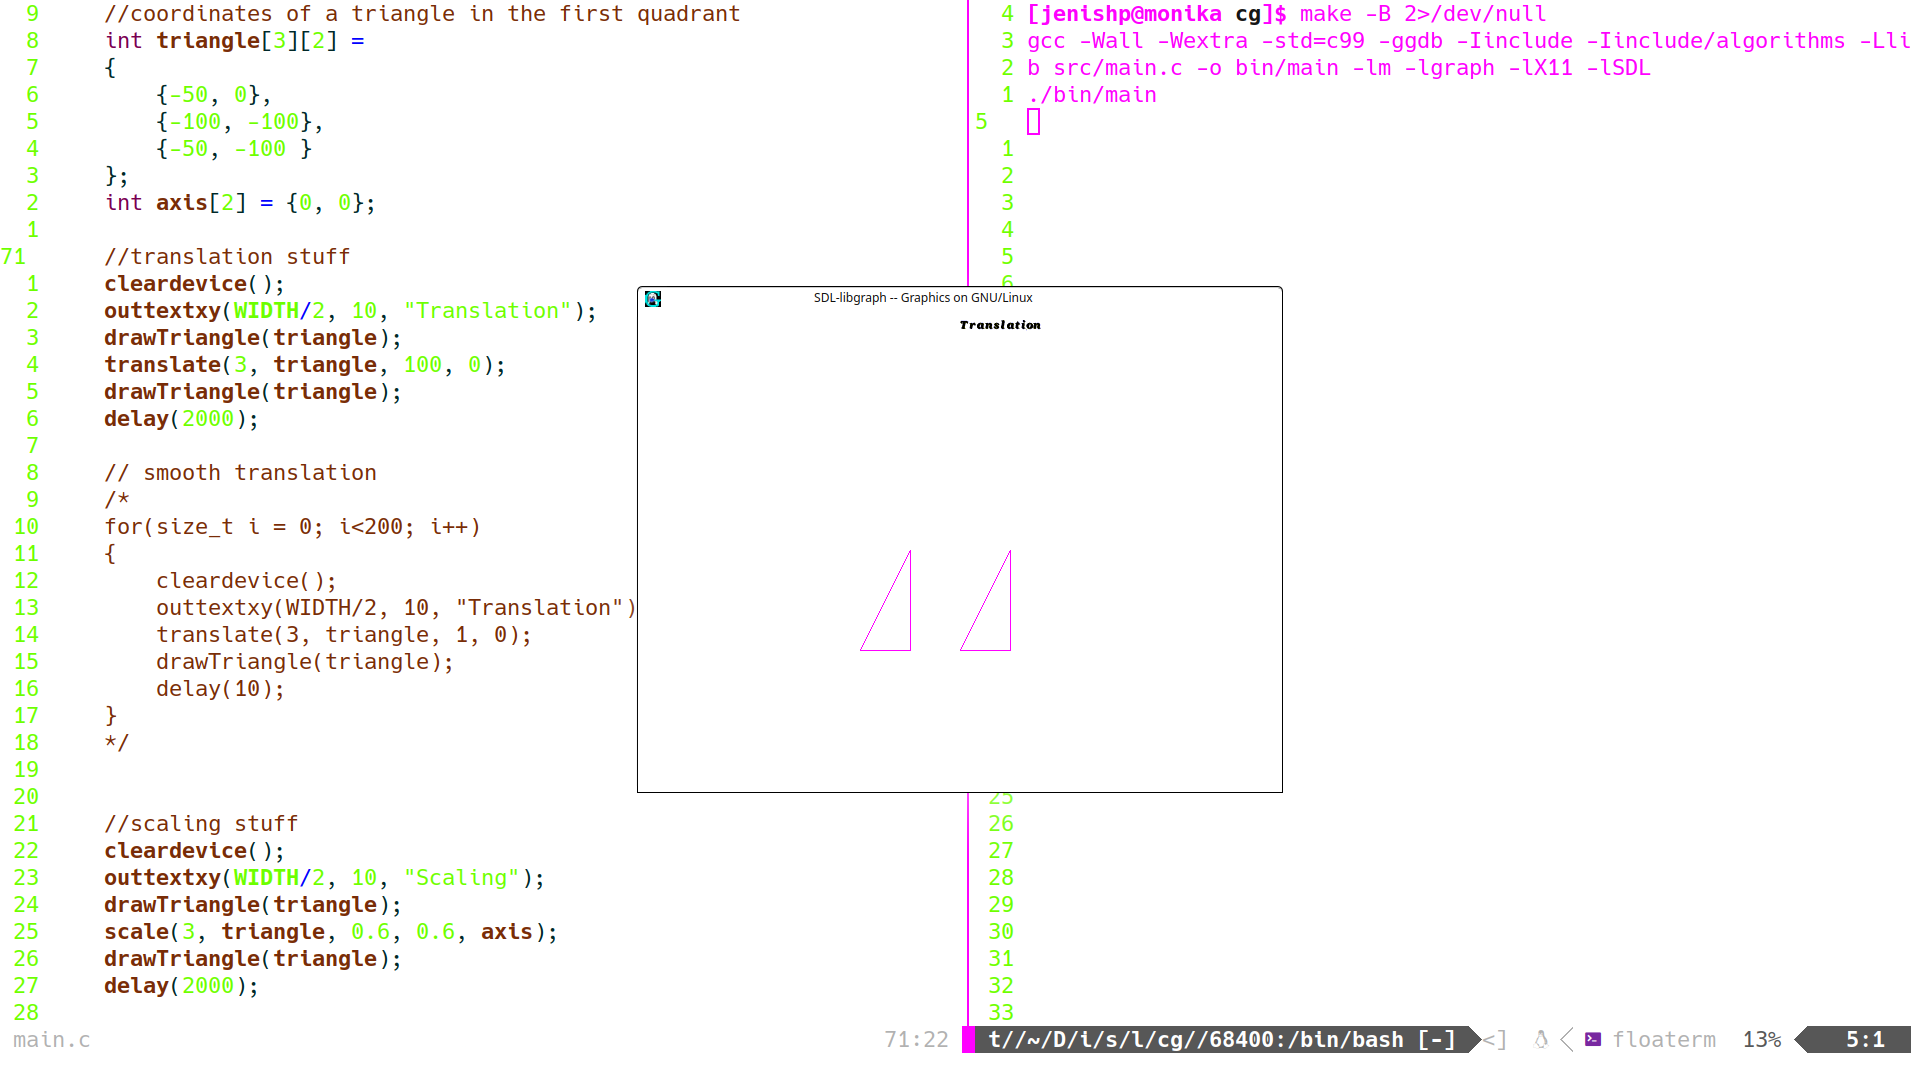
\includegraphics[width=1.01\linewidth]{translation.png}
		\caption{Translation}
		\label{fig: Translation}
	\end{figure}
	\begin{figure}[!ht]
		\hspace*{-1cm}
		\centering
		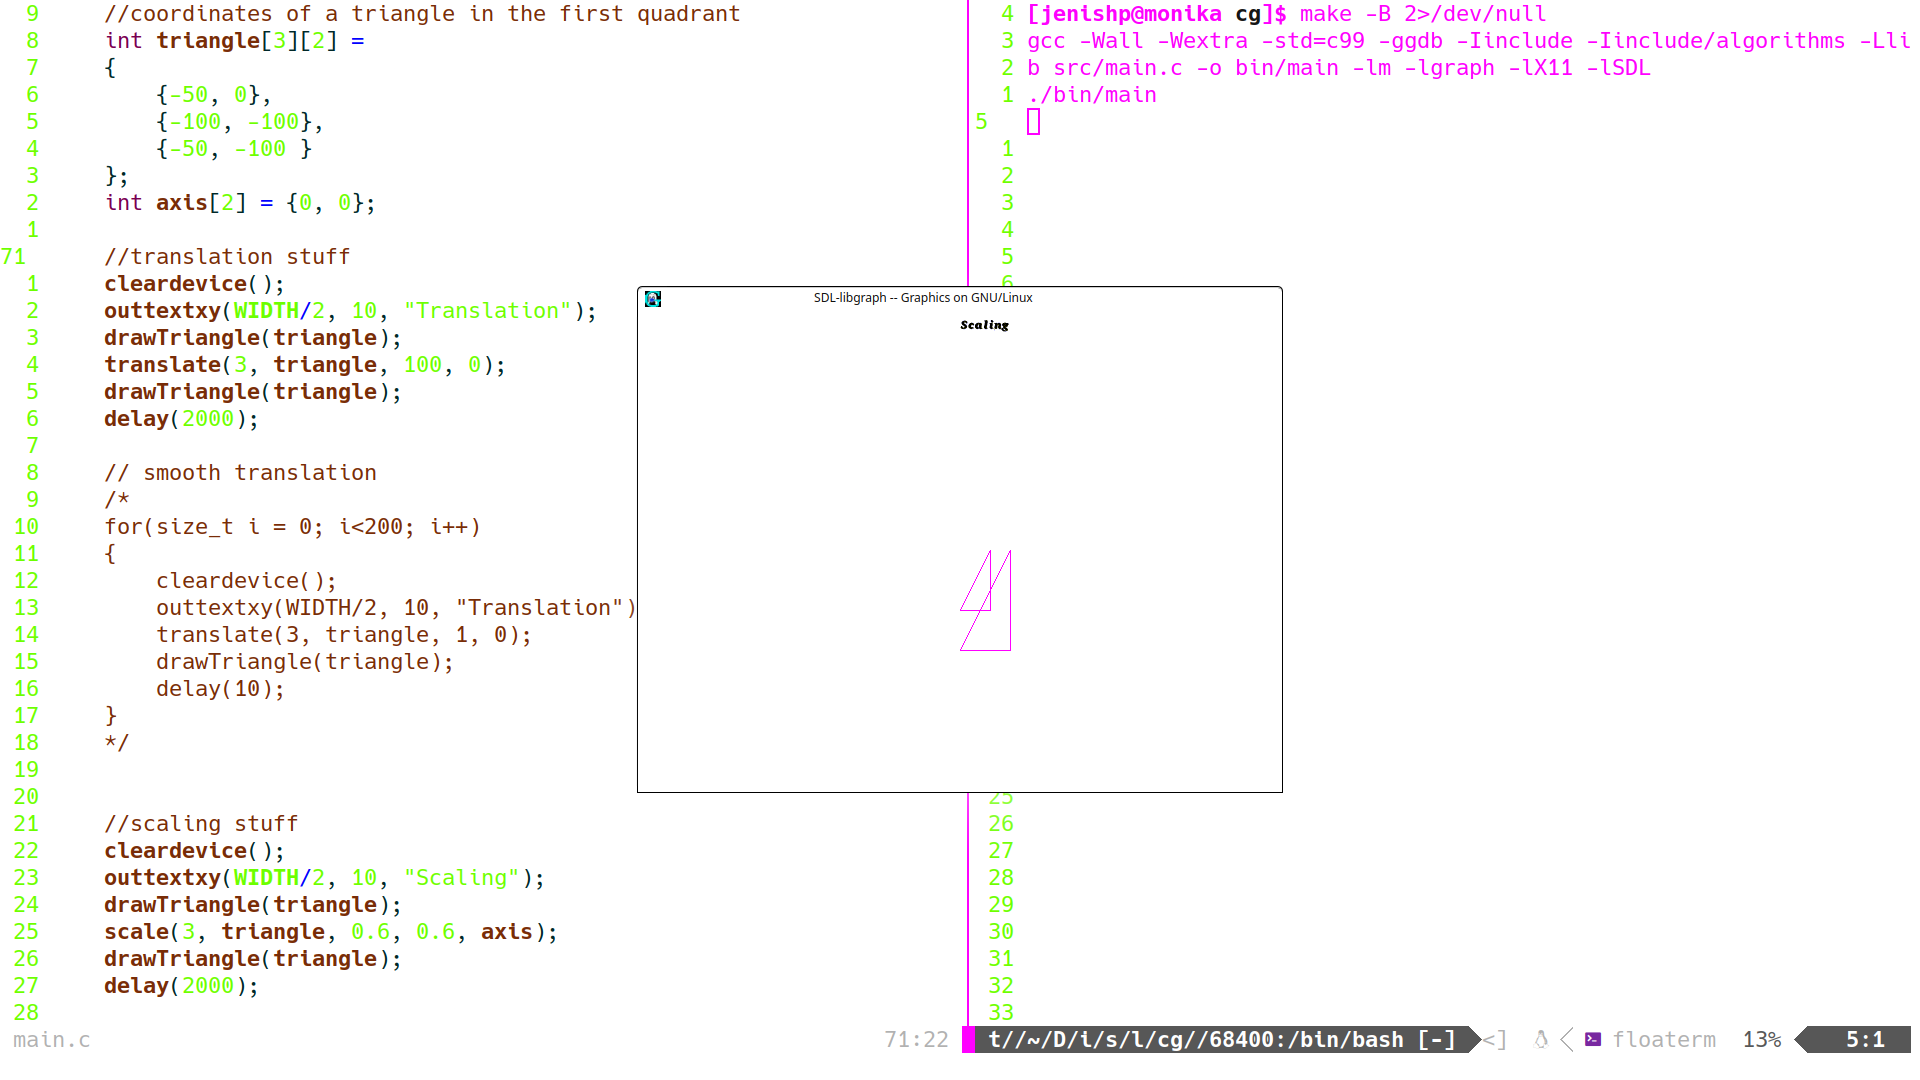
\includegraphics[width=1.01\linewidth]{scaling.png}
		\caption{Scaling}
		\label{fig: Scaling}
	\end{figure}
	\begin{figure}[!ht]
		\hspace*{-1cm}
		\centering
		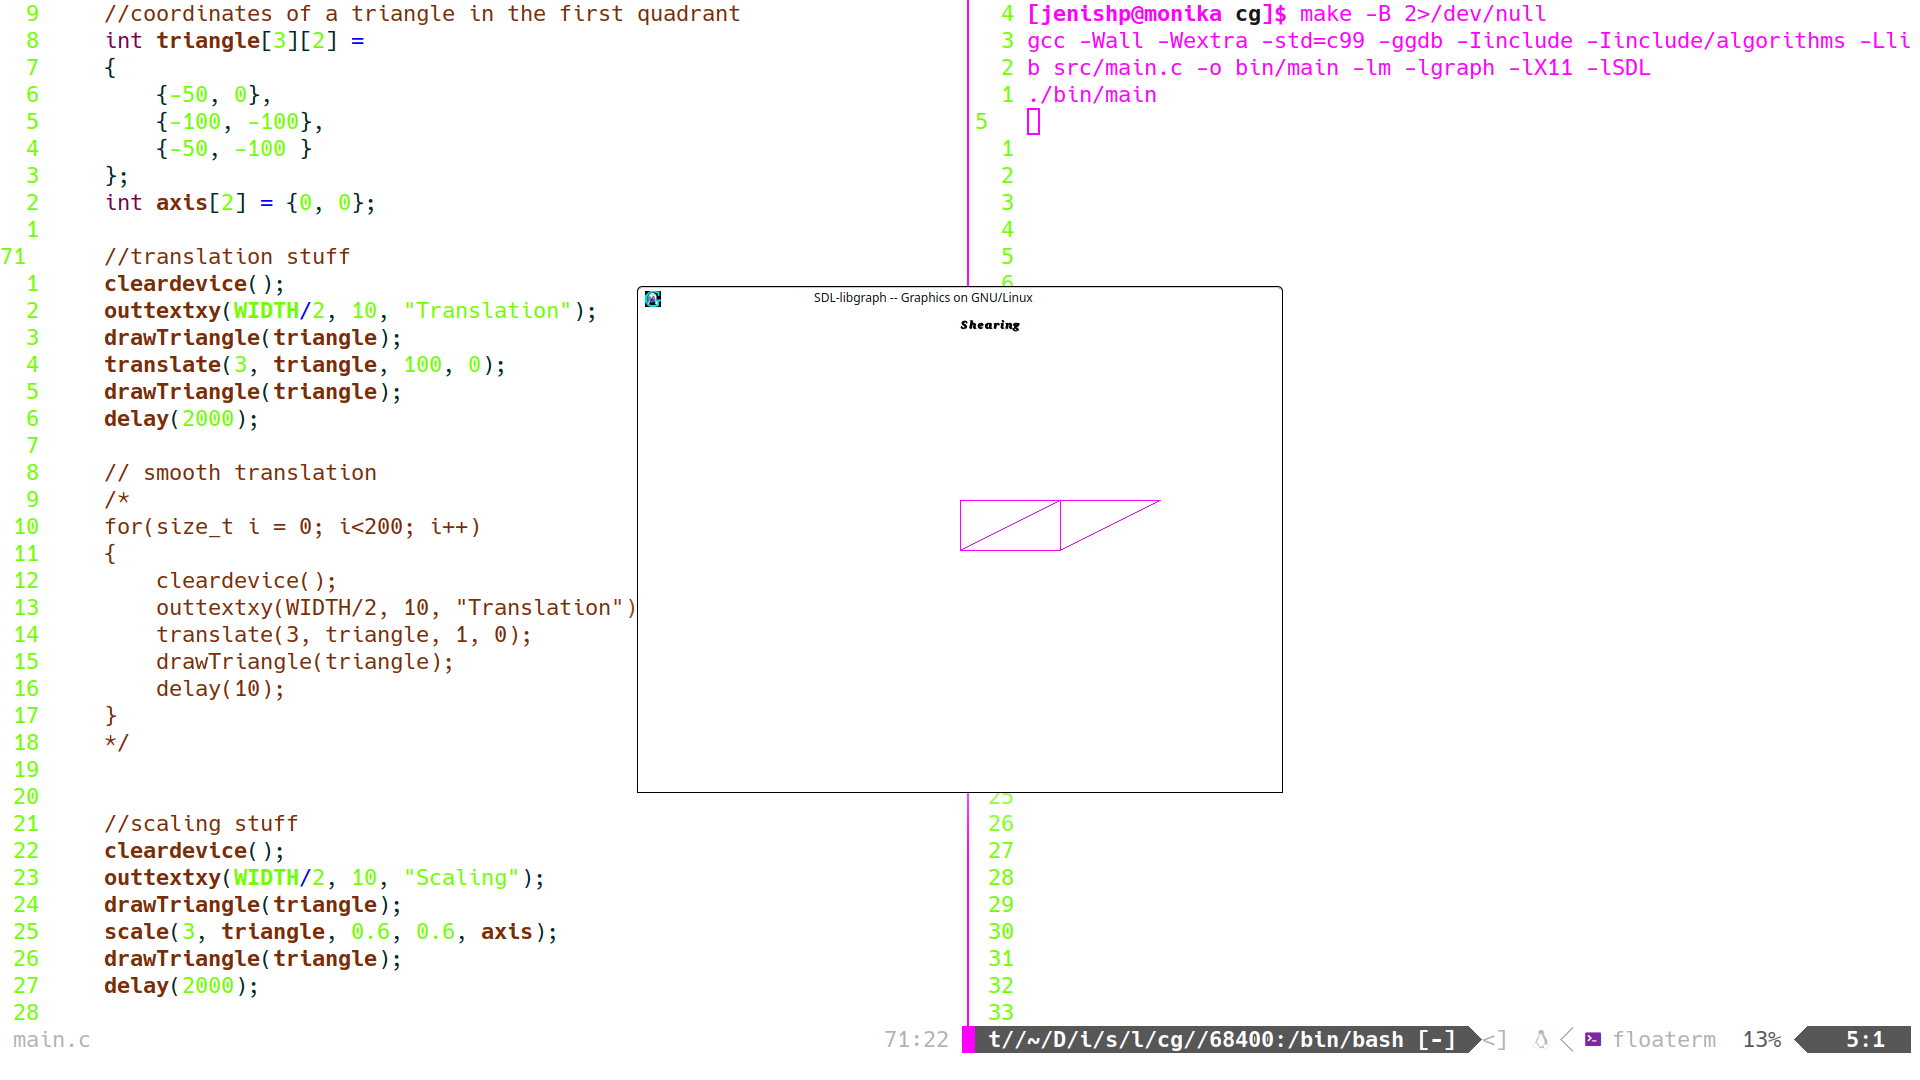
\includegraphics[width=1.01\linewidth]{shearing.png}
		\caption{Shearing}
		\label{fig: Shearing}
	\end{figure}

	\section{Conclusion}
	Given objects such as triangle and square represented by their vertices, translation, scaling and shearing were implemented on them using the graphics.h library.

\end{document}


